% Options for packages loaded elsewhere
\PassOptionsToPackage{unicode}{hyperref}
\PassOptionsToPackage{hyphens}{url}
\PassOptionsToPackage{dvipsnames,svgnames,x11names}{xcolor}
%
\documentclass[
]{article}
\usepackage{amsmath,amssymb}
\usepackage{lmodern}
\usepackage{iftex}
\ifPDFTeX
  \usepackage[T1]{fontenc}
  \usepackage[utf8]{inputenc}
  \usepackage{textcomp} % provide euro and other symbols
\else % if luatex or xetex
  \usepackage{unicode-math}
  \defaultfontfeatures{Scale=MatchLowercase}
  \defaultfontfeatures[\rmfamily]{Ligatures=TeX,Scale=1}
\fi
% Use upquote if available, for straight quotes in verbatim environments
\IfFileExists{upquote.sty}{\usepackage{upquote}}{}
\IfFileExists{microtype.sty}{% use microtype if available
  \usepackage[]{microtype}
  \UseMicrotypeSet[protrusion]{basicmath} % disable protrusion for tt fonts
}{}
\makeatletter
\@ifundefined{KOMAClassName}{% if non-KOMA class
  \IfFileExists{parskip.sty}{%
    \usepackage{parskip}
  }{% else
    \setlength{\parindent}{0pt}
    \setlength{\parskip}{6pt plus 2pt minus 1pt}}
}{% if KOMA class
  \KOMAoptions{parskip=half}}
\makeatother
\usepackage{xcolor}
\usepackage[margin=1in]{geometry}
\usepackage{color}
\usepackage{fancyvrb}
\newcommand{\VerbBar}{|}
\newcommand{\VERB}{\Verb[commandchars=\\\{\}]}
\DefineVerbatimEnvironment{Highlighting}{Verbatim}{commandchars=\\\{\}}
% Add ',fontsize=\small' for more characters per line
\usepackage{framed}
\definecolor{shadecolor}{RGB}{248,248,248}
\newenvironment{Shaded}{\begin{snugshade}}{\end{snugshade}}
\newcommand{\AlertTok}[1]{\textcolor[rgb]{0.94,0.16,0.16}{#1}}
\newcommand{\AnnotationTok}[1]{\textcolor[rgb]{0.56,0.35,0.01}{\textbf{\textit{#1}}}}
\newcommand{\AttributeTok}[1]{\textcolor[rgb]{0.77,0.63,0.00}{#1}}
\newcommand{\BaseNTok}[1]{\textcolor[rgb]{0.00,0.00,0.81}{#1}}
\newcommand{\BuiltInTok}[1]{#1}
\newcommand{\CharTok}[1]{\textcolor[rgb]{0.31,0.60,0.02}{#1}}
\newcommand{\CommentTok}[1]{\textcolor[rgb]{0.56,0.35,0.01}{\textit{#1}}}
\newcommand{\CommentVarTok}[1]{\textcolor[rgb]{0.56,0.35,0.01}{\textbf{\textit{#1}}}}
\newcommand{\ConstantTok}[1]{\textcolor[rgb]{0.00,0.00,0.00}{#1}}
\newcommand{\ControlFlowTok}[1]{\textcolor[rgb]{0.13,0.29,0.53}{\textbf{#1}}}
\newcommand{\DataTypeTok}[1]{\textcolor[rgb]{0.13,0.29,0.53}{#1}}
\newcommand{\DecValTok}[1]{\textcolor[rgb]{0.00,0.00,0.81}{#1}}
\newcommand{\DocumentationTok}[1]{\textcolor[rgb]{0.56,0.35,0.01}{\textbf{\textit{#1}}}}
\newcommand{\ErrorTok}[1]{\textcolor[rgb]{0.64,0.00,0.00}{\textbf{#1}}}
\newcommand{\ExtensionTok}[1]{#1}
\newcommand{\FloatTok}[1]{\textcolor[rgb]{0.00,0.00,0.81}{#1}}
\newcommand{\FunctionTok}[1]{\textcolor[rgb]{0.00,0.00,0.00}{#1}}
\newcommand{\ImportTok}[1]{#1}
\newcommand{\InformationTok}[1]{\textcolor[rgb]{0.56,0.35,0.01}{\textbf{\textit{#1}}}}
\newcommand{\KeywordTok}[1]{\textcolor[rgb]{0.13,0.29,0.53}{\textbf{#1}}}
\newcommand{\NormalTok}[1]{#1}
\newcommand{\OperatorTok}[1]{\textcolor[rgb]{0.81,0.36,0.00}{\textbf{#1}}}
\newcommand{\OtherTok}[1]{\textcolor[rgb]{0.56,0.35,0.01}{#1}}
\newcommand{\PreprocessorTok}[1]{\textcolor[rgb]{0.56,0.35,0.01}{\textit{#1}}}
\newcommand{\RegionMarkerTok}[1]{#1}
\newcommand{\SpecialCharTok}[1]{\textcolor[rgb]{0.00,0.00,0.00}{#1}}
\newcommand{\SpecialStringTok}[1]{\textcolor[rgb]{0.31,0.60,0.02}{#1}}
\newcommand{\StringTok}[1]{\textcolor[rgb]{0.31,0.60,0.02}{#1}}
\newcommand{\VariableTok}[1]{\textcolor[rgb]{0.00,0.00,0.00}{#1}}
\newcommand{\VerbatimStringTok}[1]{\textcolor[rgb]{0.31,0.60,0.02}{#1}}
\newcommand{\WarningTok}[1]{\textcolor[rgb]{0.56,0.35,0.01}{\textbf{\textit{#1}}}}
\usepackage{graphicx}
\makeatletter
\def\maxwidth{\ifdim\Gin@nat@width>\linewidth\linewidth\else\Gin@nat@width\fi}
\def\maxheight{\ifdim\Gin@nat@height>\textheight\textheight\else\Gin@nat@height\fi}
\makeatother
% Scale images if necessary, so that they will not overflow the page
% margins by default, and it is still possible to overwrite the defaults
% using explicit options in \includegraphics[width, height, ...]{}
\setkeys{Gin}{width=\maxwidth,height=\maxheight,keepaspectratio}
% Set default figure placement to htbp
\makeatletter
\def\fps@figure{htbp}
\makeatother
\setlength{\emergencystretch}{3em} % prevent overfull lines
\providecommand{\tightlist}{%
  \setlength{\itemsep}{0pt}\setlength{\parskip}{0pt}}
\setcounter{secnumdepth}{-\maxdimen} % remove section numbering
\ifLuaTeX
  \usepackage{selnolig}  % disable illegal ligatures
\fi
\IfFileExists{bookmark.sty}{\usepackage{bookmark}}{\usepackage{hyperref}}
\IfFileExists{xurl.sty}{\usepackage{xurl}}{} % add URL line breaks if available
\urlstyle{same} % disable monospaced font for URLs
\hypersetup{
  pdftitle={Module 2: Recommended Exercises - Solution},
  pdfauthor={Emma Skarstein, Daesoo Lee, Kenneth Aase, Stefanie Muff; Department of Mathematical Sciences, NTNU},
  colorlinks=true,
  linkcolor={Maroon},
  filecolor={Maroon},
  citecolor={Blue},
  urlcolor={blue},
  pdfcreator={LaTeX via pandoc}}

\title{Module 2: Recommended Exercises - Solution}
\usepackage{etoolbox}
\makeatletter
\providecommand{\subtitle}[1]{% add subtitle to \maketitle
  \apptocmd{\@title}{\par {\large #1 \par}}{}{}
}
\makeatother
\subtitle{TMA4268 Statistical Learning V2023}
\author{Emma Skarstein, Daesoo Lee, Kenneth Aase, Stefanie
Muff \and Department of Mathematical Sciences, NTNU}
\date{January 19, 2023}

\begin{document}
\maketitle

Last changes: 2023-01-10

\begin{center}\rule{0.5\linewidth}{0.5pt}\end{center}

\hypertarget{problem-1}{%
\section{Problem 1}\label{problem-1}}

\begin{enumerate}
\def\labelenumi{\alph{enumi})}
\item
  Classification

  Example 1: Cancer diagnostics. Response: cancer (yes/no). Predictors:
  smoking, age, family history, gene expression ect. Goal: prediction.

  Example 2: Stock market price direction. Response: up/down.
  Predictors: yesterday's price movement change, two previous days price
  movement ect. Goal: inference.

  Example 3: Flower species. Response: species. Predictors: color,
  height, leafes ect. Goal: prediction
\item
  Regression

  Example 1: Illness classification. Response: age of death. Predictors:
  current age, gender, resting heart rate, resting breath rate ect.
  Goal: prediction

  Example 2: House price. Response: Price. Predictors: age of house,
  price of neighbourhood, crime rate, distance to town, distance to
  school, ect. Goal: prediction

  Example 3: What affects O2-uptake. Response: O2-uptake. Predictors:
  gender, age, amount of weekly exercise, type of exercise, smoking,
  heart disease, ect. Goal: inference
\end{enumerate}

\hypertarget{problem-2}{%
\section{Problem 2}\label{problem-2}}

\begin{enumerate}
\def\labelenumi{\alph{enumi})}
\tightlist
\item
  Based on the three different models compared here, a rigid method will
  have the highest test MSE. However, this does not always have to be
  the case. For instance, in figure 2.10, we see that the most flexible
  model has the highest test MSE. See also figure 2.12 that summarizes
  the last three figures and shows some of the variation. So in general
  we cannot say anything certain about how the test MSE will vary based
  on model flexibility, this will depend on how the training data
  compares to the test data, and other model characteristics. However
  (though the question does not ask this), the \emph{training} MSE will
  always decrease as the flexibility increases.
\item
  A small (test) variance implies an underfit to the data.
\item
  See figure 2.12. Underfit - low variance - high bias. Overfit - high
  variance - low bias. We wish to find a model that lies somewhere
  inbetween, with low variance and low bias.
\end{enumerate}

\hypertarget{problem-3}{%
\section{Problem 3}\label{problem-3}}

\begin{Shaded}
\begin{Highlighting}[]
\CommentTok{\#install.packages("ISLR")}
\FunctionTok{library}\NormalTok{(ISLR)}
\FunctionTok{data}\NormalTok{(Auto)}
\end{Highlighting}
\end{Shaded}

\begin{enumerate}
\def\labelenumi{\alph{enumi})}
\tightlist
\item
\end{enumerate}

\begin{Shaded}
\begin{Highlighting}[]
\FunctionTok{str}\NormalTok{(Auto)}
\end{Highlighting}
\end{Shaded}

\begin{verbatim}
## 'data.frame':    392 obs. of  9 variables:
##  $ mpg         : num  18 15 18 16 17 15 14 14 14 15 ...
##  $ cylinders   : num  8 8 8 8 8 8 8 8 8 8 ...
##  $ displacement: num  307 350 318 304 302 429 454 440 455 390 ...
##  $ horsepower  : num  130 165 150 150 140 198 220 215 225 190 ...
##  $ weight      : num  3504 3693 3436 3433 3449 ...
##  $ acceleration: num  12 11.5 11 12 10.5 10 9 8.5 10 8.5 ...
##  $ year        : num  70 70 70 70 70 70 70 70 70 70 ...
##  $ origin      : num  1 1 1 1 1 1 1 1 1 1 ...
##  $ name        : Factor w/ 304 levels "amc ambassador brougham",..: 49 36 231 14 161 141 54 223 241 2 ...
\end{verbatim}

\begin{Shaded}
\begin{Highlighting}[]
\FunctionTok{summary}\NormalTok{(Auto)}
\end{Highlighting}
\end{Shaded}

\begin{verbatim}
##       mpg          cylinders      displacement     horsepower        weight      acceleration  
##  Min.   : 9.00   Min.   :3.000   Min.   : 68.0   Min.   : 46.0   Min.   :1613   Min.   : 8.00  
##  1st Qu.:17.00   1st Qu.:4.000   1st Qu.:105.0   1st Qu.: 75.0   1st Qu.:2225   1st Qu.:13.78  
##  Median :22.75   Median :4.000   Median :151.0   Median : 93.5   Median :2804   Median :15.50  
##  Mean   :23.45   Mean   :5.472   Mean   :194.4   Mean   :104.5   Mean   :2978   Mean   :15.54  
##  3rd Qu.:29.00   3rd Qu.:8.000   3rd Qu.:275.8   3rd Qu.:126.0   3rd Qu.:3615   3rd Qu.:17.02  
##  Max.   :46.60   Max.   :8.000   Max.   :455.0   Max.   :230.0   Max.   :5140   Max.   :24.80  
##                                                                                                
##       year           origin                      name    
##  Min.   :70.00   Min.   :1.000   amc matador       :  5  
##  1st Qu.:73.00   1st Qu.:1.000   ford pinto        :  5  
##  Median :76.00   Median :1.000   toyota corolla    :  5  
##  Mean   :75.98   Mean   :1.577   amc gremlin       :  4  
##  3rd Qu.:79.00   3rd Qu.:2.000   amc hornet        :  4  
##  Max.   :82.00   Max.   :3.000   chevrolet chevette:  4  
##                                  (Other)           :365
\end{verbatim}

The dimensions are 392 observations (rows) of 9 variables (columns). See
from looking at the structure (\texttt{str()}) and \texttt{summary()}
that cylinders (taking values 3,4,5,6,8), origin (taking values 1,2,3)
and name (name of the cars) are qualitative predictors. The rest of the
predictors are quantitative.

\begin{enumerate}
\def\labelenumi{\alph{enumi})}
\setcounter{enumi}{1}
\tightlist
\item
  To see the range of the quantitative predictors, either apply the
  \texttt{range()} function to each column with a quantitative predictor
  separately
\end{enumerate}

\begin{Shaded}
\begin{Highlighting}[]
\FunctionTok{range}\NormalTok{(Auto[,}\DecValTok{1}\NormalTok{])}
\end{Highlighting}
\end{Shaded}

\begin{verbatim}
## [1]  9.0 46.6
\end{verbatim}

\begin{Shaded}
\begin{Highlighting}[]
\FunctionTok{range}\NormalTok{(Auto[,}\DecValTok{3}\NormalTok{])}
\end{Highlighting}
\end{Shaded}

\begin{verbatim}
## [1]  68 455
\end{verbatim}

\begin{Shaded}
\begin{Highlighting}[]
\FunctionTok{range}\NormalTok{(Auto[,}\DecValTok{4}\NormalTok{])}
\end{Highlighting}
\end{Shaded}

\begin{verbatim}
## [1]  46 230
\end{verbatim}

\begin{Shaded}
\begin{Highlighting}[]
\FunctionTok{range}\NormalTok{(Auto[,}\DecValTok{5}\NormalTok{])}
\end{Highlighting}
\end{Shaded}

\begin{verbatim}
## [1] 1613 5140
\end{verbatim}

\begin{Shaded}
\begin{Highlighting}[]
\FunctionTok{range}\NormalTok{(Auto[,}\DecValTok{6}\NormalTok{])}
\end{Highlighting}
\end{Shaded}

\begin{verbatim}
## [1]  8.0 24.8
\end{verbatim}

\begin{Shaded}
\begin{Highlighting}[]
\FunctionTok{range}\NormalTok{(Auto[,}\DecValTok{7}\NormalTok{])}
\end{Highlighting}
\end{Shaded}

\begin{verbatim}
## [1] 70 82
\end{verbatim}

or use the \texttt{sapply()} function to run the \texttt{range()}
function on the specified columns with a single line of code:

\begin{Shaded}
\begin{Highlighting}[]
\NormalTok{quant }\OtherTok{=} \FunctionTok{c}\NormalTok{(}\DecValTok{1}\NormalTok{,}\DecValTok{3}\NormalTok{,}\DecValTok{4}\NormalTok{,}\DecValTok{5}\NormalTok{,}\DecValTok{6}\NormalTok{,}\DecValTok{7}\NormalTok{)}
\FunctionTok{sapply}\NormalTok{(Auto[, quant], range)}
\end{Highlighting}
\end{Shaded}

\begin{verbatim}
##       mpg displacement horsepower weight acceleration year
## [1,]  9.0           68         46   1613          8.0   70
## [2,] 46.6          455        230   5140         24.8   82
\end{verbatim}

\begin{enumerate}
\def\labelenumi{\alph{enumi})}
\setcounter{enumi}{2}
\tightlist
\item
  To get the and standard deviation of the quantitative predictors, we
  can again either use the \texttt{sapply()} function in the same manner
  as above, or apply the \texttt{mean()} and \texttt{sd()} commands
  columnwise.
\end{enumerate}

\begin{Shaded}
\begin{Highlighting}[]
\CommentTok{\#mean}
\FunctionTok{sapply}\NormalTok{(Auto[, quant], mean)}
\end{Highlighting}
\end{Shaded}

\begin{verbatim}
##          mpg displacement   horsepower       weight acceleration         year 
##     23.44592    194.41199    104.46939   2977.58418     15.54133     75.97959
\end{verbatim}

\begin{Shaded}
\begin{Highlighting}[]
\CommentTok{\#or}
\FunctionTok{mean}\NormalTok{(Auto[,}\DecValTok{1}\NormalTok{])}
\end{Highlighting}
\end{Shaded}

\begin{verbatim}
## [1] 23.44592
\end{verbatim}

\begin{Shaded}
\begin{Highlighting}[]
\FunctionTok{mean}\NormalTok{(Auto[,}\DecValTok{3}\NormalTok{])}
\end{Highlighting}
\end{Shaded}

\begin{verbatim}
## [1] 194.412
\end{verbatim}

\begin{Shaded}
\begin{Highlighting}[]
\FunctionTok{mean}\NormalTok{(Auto[,}\DecValTok{4}\NormalTok{])}
\end{Highlighting}
\end{Shaded}

\begin{verbatim}
## [1] 104.4694
\end{verbatim}

\begin{Shaded}
\begin{Highlighting}[]
\FunctionTok{mean}\NormalTok{(Auto[,}\DecValTok{5}\NormalTok{])}
\end{Highlighting}
\end{Shaded}

\begin{verbatim}
## [1] 2977.584
\end{verbatim}

\begin{Shaded}
\begin{Highlighting}[]
\FunctionTok{mean}\NormalTok{(Auto[,}\DecValTok{6}\NormalTok{])}
\end{Highlighting}
\end{Shaded}

\begin{verbatim}
## [1] 15.54133
\end{verbatim}

\begin{Shaded}
\begin{Highlighting}[]
\FunctionTok{mean}\NormalTok{(Auto[,}\DecValTok{7}\NormalTok{])}
\end{Highlighting}
\end{Shaded}

\begin{verbatim}
## [1] 75.97959
\end{verbatim}

\begin{Shaded}
\begin{Highlighting}[]
\CommentTok{\#or}
\FunctionTok{colMeans}\NormalTok{(Auto[,quant])}
\end{Highlighting}
\end{Shaded}

\begin{verbatim}
##          mpg displacement   horsepower       weight acceleration         year 
##     23.44592    194.41199    104.46939   2977.58418     15.54133     75.97959
\end{verbatim}

\begin{Shaded}
\begin{Highlighting}[]
\CommentTok{\#sd}
\FunctionTok{sapply}\NormalTok{(Auto[, quant], sd)}
\end{Highlighting}
\end{Shaded}

\begin{verbatim}
##          mpg displacement   horsepower       weight acceleration         year 
##     7.805007   104.644004    38.491160   849.402560     2.758864     3.683737
\end{verbatim}

\begin{Shaded}
\begin{Highlighting}[]
\CommentTok{\#or}
\FunctionTok{sd}\NormalTok{(Auto[,}\DecValTok{1}\NormalTok{])}
\end{Highlighting}
\end{Shaded}

\begin{verbatim}
## [1] 7.805007
\end{verbatim}

\begin{Shaded}
\begin{Highlighting}[]
\FunctionTok{sd}\NormalTok{(Auto[,}\DecValTok{3}\NormalTok{])}
\end{Highlighting}
\end{Shaded}

\begin{verbatim}
## [1] 104.644
\end{verbatim}

\begin{Shaded}
\begin{Highlighting}[]
\FunctionTok{sd}\NormalTok{(Auto[,}\DecValTok{4}\NormalTok{])}
\end{Highlighting}
\end{Shaded}

\begin{verbatim}
## [1] 38.49116
\end{verbatim}

\begin{Shaded}
\begin{Highlighting}[]
\FunctionTok{sd}\NormalTok{(Auto[,}\DecValTok{5}\NormalTok{])}
\end{Highlighting}
\end{Shaded}

\begin{verbatim}
## [1] 849.4026
\end{verbatim}

\begin{Shaded}
\begin{Highlighting}[]
\FunctionTok{sd}\NormalTok{(Auto[,}\DecValTok{6}\NormalTok{])}
\end{Highlighting}
\end{Shaded}

\begin{verbatim}
## [1] 2.758864
\end{verbatim}

\begin{Shaded}
\begin{Highlighting}[]
\FunctionTok{sd}\NormalTok{(Auto[,}\DecValTok{7}\NormalTok{])}
\end{Highlighting}
\end{Shaded}

\begin{verbatim}
## [1] 3.683737
\end{verbatim}

\begin{enumerate}
\def\labelenumi{\alph{enumi})}
\setcounter{enumi}{3}
\tightlist
\item
  Remove 10th to 85th observations and look at the range, mean and
  standard deviation of the reduced set. We now only show the solutions
  using \texttt{sapply()} to save space.
\end{enumerate}

\begin{Shaded}
\begin{Highlighting}[]
\CommentTok{\#remove observations}
\NormalTok{ReducedAuto }\OtherTok{=}\NormalTok{ Auto[}\SpecialCharTok{{-}}\FunctionTok{c}\NormalTok{(}\DecValTok{10}\SpecialCharTok{:}\DecValTok{85}\NormalTok{),]}

\CommentTok{\#range, mean and sd}
\FunctionTok{sapply}\NormalTok{(ReducedAuto[, quant], range)}
\end{Highlighting}
\end{Shaded}

\begin{verbatim}
##       mpg displacement horsepower weight acceleration year
## [1,] 11.0           68         46   1649          8.5   70
## [2,] 46.6          455        230   4997         24.8   82
\end{verbatim}

\begin{Shaded}
\begin{Highlighting}[]
\FunctionTok{sapply}\NormalTok{(ReducedAuto[, quant], mean)}
\end{Highlighting}
\end{Shaded}

\begin{verbatim}
##          mpg displacement   horsepower       weight acceleration         year 
##     24.40443    187.24051    100.72152   2935.97152     15.72690     77.14557
\end{verbatim}

\begin{Shaded}
\begin{Highlighting}[]
\FunctionTok{sapply}\NormalTok{(ReducedAuto[, quant], sd)}
\end{Highlighting}
\end{Shaded}

\begin{verbatim}
##          mpg displacement   horsepower       weight acceleration         year 
##     7.867283    99.678367    35.708853   811.300208     2.693721     3.106217
\end{verbatim}

\begin{enumerate}
\def\labelenumi{\alph{enumi})}
\setcounter{enumi}{4}
\tightlist
\item
  Make a scatterplot of the full dataset using the \texttt{ggpairs()}
  function.
\end{enumerate}

\begin{Shaded}
\begin{Highlighting}[]
\FunctionTok{library}\NormalTok{(GGally)}
\FunctionTok{ggpairs}\NormalTok{(Auto[,quant]) }\SpecialCharTok{+} \FunctionTok{theme\_minimal}\NormalTok{()}
\end{Highlighting}
\end{Shaded}

\begin{verbatim}
## plot: [1,1] [=>-------------------------------------------------------------------------] 3% est: 0s
## plot: [1,2] [===>-----------------------------------------------------------------------] 6% est: 1s
## plot: [1,3] [=====>---------------------------------------------------------------------] 8% est: 1s
## plot: [1,4] [=======>-------------------------------------------------------------------] 11% est: 1s
## plot: [1,5] [=========>-----------------------------------------------------------------] 14% est: 1s
## plot: [1,6] [===========>---------------------------------------------------------------] 17% est: 1s
## plot: [2,1] [==============>------------------------------------------------------------] 19% est: 1s
## plot: [2,2] [================>----------------------------------------------------------] 22% est: 1s
## plot: [2,3] [==================>--------------------------------------------------------] 25% est: 1s
## plot: [2,4] [====================>------------------------------------------------------] 28% est: 1s
## plot: [2,5] [======================>----------------------------------------------------] 31% est: 1s
## plot: [2,6] [========================>--------------------------------------------------] 33% est: 1s
## plot: [3,1] [==========================>------------------------------------------------] 36% est: 1s
## plot: [3,2] [============================>----------------------------------------------] 39% est: 1s
## plot: [3,3] [==============================>--------------------------------------------] 42% est: 1s
## plot: [3,4] [================================>------------------------------------------] 44% est: 1s
## plot: [3,5] [==================================>----------------------------------------] 47% est: 1s
## plot: [3,6] [=====================================>-------------------------------------] 50% est: 1s
## plot: [4,1] [=======================================>-----------------------------------] 53% est: 1s
## plot: [4,2] [=========================================>---------------------------------] 56% est: 1s
## plot: [4,3] [===========================================>-------------------------------] 58% est: 1s
## plot: [4,4] [=============================================>-----------------------------] 61% est: 1s
## plot: [4,5] [===============================================>---------------------------] 64% est: 1s
## plot: [4,6] [=================================================>-------------------------] 67% est: 1s
## plot: [5,1] [===================================================>-----------------------] 69% est: 0s
## plot: [5,2] [=====================================================>---------------------] 72% est: 0s
## plot: [5,3] [=======================================================>-------------------] 75% est: 0s
## plot: [5,4] [=========================================================>-----------------] 78% est: 0s
## plot: [5,5] [===========================================================>---------------] 81% est: 0s
## plot: [5,6] [=============================================================>-------------] 83% est: 0s
## plot: [6,1] [================================================================>----------] 86% est: 0s
## plot: [6,2] [==================================================================>--------] 89% est: 0s
## plot: [6,3] [====================================================================>------] 92% est: 0s
## plot: [6,4] [======================================================================>----] 94% est: 0s
## plot: [6,5] [========================================================================>--] 97% est: 0s
## plot: [6,6] [===========================================================================]100% est: 0s
\end{verbatim}

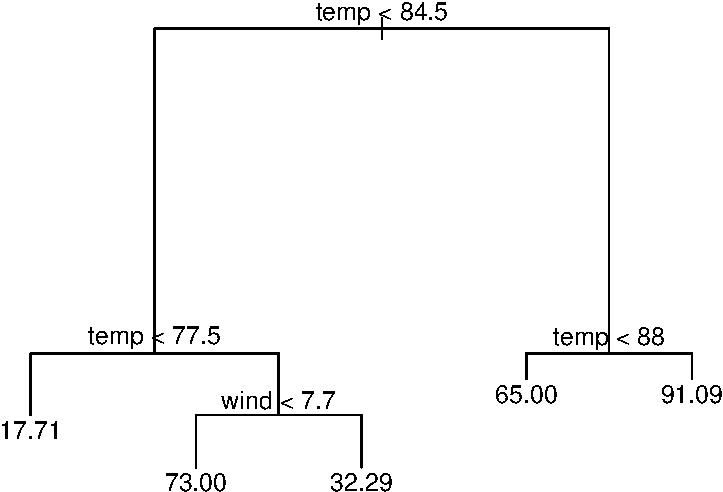
\includegraphics{RecEx2-sol_files/figure-latex/unnamed-chunk-7-1.pdf}

We see that there seems to be strong relationships (based on curve
trends and correlation) between the pairs: \texttt{mpg} and
\texttt{displacement}, \texttt{mpg} and \texttt{horsepower},
\texttt{mpg} and \texttt{weight}, \texttt{displacement} and
\texttt{horsepower}, \texttt{displacement} and \texttt{weight},
\texttt{horsepower} and \texttt{weght}, and \texttt{horsepower} and
\texttt{acceleration}.

\begin{enumerate}
\def\labelenumi{\alph{enumi})}
\setcounter{enumi}{5}
\tightlist
\item
  Wish to predict gas milage based on the other variables. From the
  scatterplot we see that \texttt{displacement}, \texttt{horsepower} and
  \texttt{weight} could be good choises for prediction of \texttt{mpg}.
  Check if the qualitative predictors could also be good choises by
  plotting them against \texttt{mpg}.
\end{enumerate}

\begin{Shaded}
\begin{Highlighting}[]
\FunctionTok{ggplot}\NormalTok{(Auto, }\FunctionTok{aes}\NormalTok{(}\FunctionTok{as.factor}\NormalTok{(cylinders), mpg)) }\SpecialCharTok{+} 
  \FunctionTok{geom\_boxplot}\NormalTok{(}\AttributeTok{fill=}\StringTok{"skyblue"}\NormalTok{) }\SpecialCharTok{+} 
  \FunctionTok{labs}\NormalTok{(}\AttributeTok{title =} \StringTok{"mgp vs cylinders"}\NormalTok{) }
\end{Highlighting}
\end{Shaded}

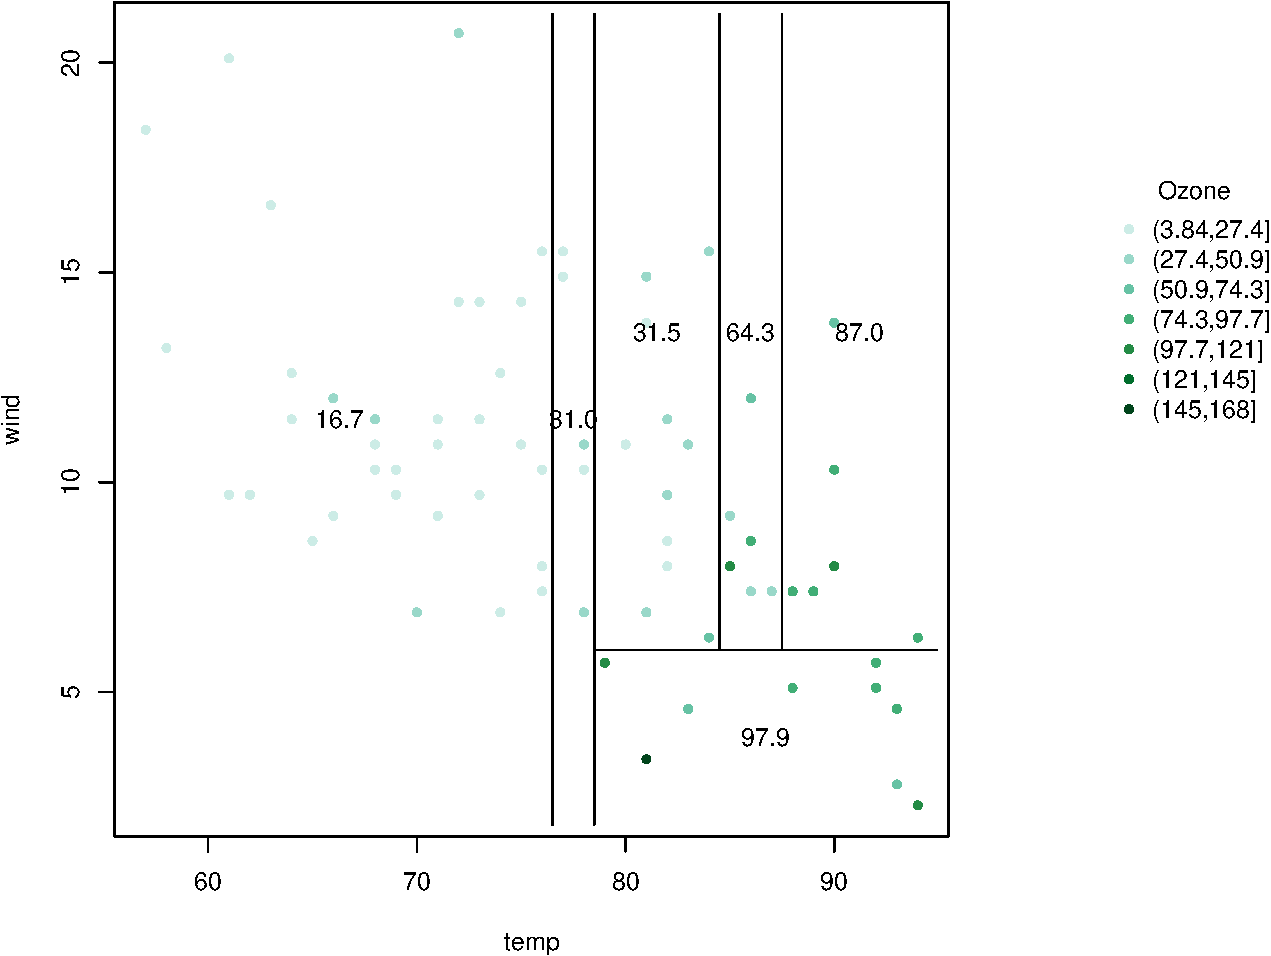
\includegraphics{RecEx2-sol_files/figure-latex/unnamed-chunk-8-1.pdf}

\begin{Shaded}
\begin{Highlighting}[]
\FunctionTok{ggplot}\NormalTok{(Auto, }\FunctionTok{aes}\NormalTok{(}\FunctionTok{as.factor}\NormalTok{(origin), mpg)) }\SpecialCharTok{+} 
  \FunctionTok{geom\_boxplot}\NormalTok{(}\AttributeTok{fill=}\StringTok{"skyblue"}\NormalTok{) }\SpecialCharTok{+} 
  \FunctionTok{labs}\NormalTok{(}\AttributeTok{title =} \StringTok{"mgp vs origin"}\NormalTok{) }
\end{Highlighting}
\end{Shaded}

\includegraphics{RecEx2-sol_files/figure-latex/unnamed-chunk-8-2.pdf}

From these plots we see that both \texttt{cylinders} and \texttt{origin}
could be good choices for prediction of \texttt{mgp}, because the miles
per gallon (mpg) seems to depend on these two variables.

\begin{enumerate}
\def\labelenumi{\alph{enumi})}
\setcounter{enumi}{6}
\tightlist
\item
  To find the correlation of the given variables, we need the covariance
  of these variable as well as the standard deviations, which are both
  available in the covariance matrix. Remember the the variance of each
  variable is given in the diagonal of the covariance matrix.
\end{enumerate}

\begin{Shaded}
\begin{Highlighting}[]
\NormalTok{covMat }\OtherTok{=} \FunctionTok{cov}\NormalTok{(Auto[,quant])}
\NormalTok{covMat[}\DecValTok{1}\NormalTok{,}\DecValTok{2}\NormalTok{]}\SpecialCharTok{/}\NormalTok{(}\FunctionTok{sqrt}\NormalTok{(covMat[}\DecValTok{1}\NormalTok{,}\DecValTok{1}\NormalTok{])}\SpecialCharTok{*}\FunctionTok{sqrt}\NormalTok{(covMat[}\DecValTok{2}\NormalTok{,}\DecValTok{2}\NormalTok{]))}
\end{Highlighting}
\end{Shaded}

\begin{verbatim}
## [1] -0.8051269
\end{verbatim}

\begin{Shaded}
\begin{Highlighting}[]
\NormalTok{covMat[}\DecValTok{1}\NormalTok{,}\DecValTok{3}\NormalTok{]}\SpecialCharTok{/}\NormalTok{(}\FunctionTok{sqrt}\NormalTok{(covMat[}\DecValTok{1}\NormalTok{,}\DecValTok{1}\NormalTok{])}\SpecialCharTok{*}\FunctionTok{sqrt}\NormalTok{(covMat[}\DecValTok{3}\NormalTok{,}\DecValTok{3}\NormalTok{]))}
\end{Highlighting}
\end{Shaded}

\begin{verbatim}
## [1] -0.7784268
\end{verbatim}

\begin{Shaded}
\begin{Highlighting}[]
\NormalTok{covMat[}\DecValTok{1}\NormalTok{,}\DecValTok{4}\NormalTok{]}\SpecialCharTok{/}\NormalTok{(}\FunctionTok{sqrt}\NormalTok{(covMat[}\DecValTok{1}\NormalTok{,}\DecValTok{1}\NormalTok{])}\SpecialCharTok{*}\FunctionTok{sqrt}\NormalTok{(covMat[}\DecValTok{4}\NormalTok{,}\DecValTok{4}\NormalTok{]))}
\end{Highlighting}
\end{Shaded}

\begin{verbatim}
## [1] -0.8322442
\end{verbatim}

\begin{Shaded}
\begin{Highlighting}[]
\FunctionTok{cor}\NormalTok{(Auto[,quant])}
\end{Highlighting}
\end{Shaded}

\begin{verbatim}
##                     mpg displacement horsepower     weight acceleration       year
## mpg           1.0000000   -0.8051269 -0.7784268 -0.8322442    0.4233285  0.5805410
## displacement -0.8051269    1.0000000  0.8972570  0.9329944   -0.5438005 -0.3698552
## horsepower   -0.7784268    0.8972570  1.0000000  0.8645377   -0.6891955 -0.4163615
## weight       -0.8322442    0.9329944  0.8645377  1.0000000   -0.4168392 -0.3091199
## acceleration  0.4233285   -0.5438005 -0.6891955 -0.4168392    1.0000000  0.2903161
## year          0.5805410   -0.3698552 -0.4163615 -0.3091199    0.2903161  1.0000000
\end{verbatim}

We see that the obtained correlations coincide with the given elements
in the correlation matrix.

\hypertarget{problem-4}{%
\section{Problem 4}\label{problem-4}}

\begin{enumerate}
\def\labelenumi{\alph{enumi})}
\tightlist
\item
  Simulate values from the four multivariate distributions using
  \texttt{mvnorm()}.
\end{enumerate}

\begin{Shaded}
\begin{Highlighting}[]
\CommentTok{\# simulate 1000 values from the multivariate normal distribution with mean = c(2,3) and cov(1,0,0,1)}
\FunctionTok{library}\NormalTok{(MASS)}
\NormalTok{set1 }\OtherTok{=} \FunctionTok{as.data.frame}\NormalTok{(}\FunctionTok{mvrnorm}\NormalTok{(}\AttributeTok{n =} \DecValTok{1000}\NormalTok{, }\AttributeTok{mu=}\FunctionTok{c}\NormalTok{(}\DecValTok{2}\NormalTok{,}\DecValTok{3}\NormalTok{), }\AttributeTok{Sigma =} \FunctionTok{matrix}\NormalTok{(}\FunctionTok{c}\NormalTok{(}\DecValTok{1}\NormalTok{,}\DecValTok{0}\NormalTok{,}\DecValTok{0}\NormalTok{,}\DecValTok{1}\NormalTok{), }\AttributeTok{ncol=}\DecValTok{2}\NormalTok{)))}
\FunctionTok{colnames}\NormalTok{(set1) }\OtherTok{=} \FunctionTok{c}\NormalTok{(}\StringTok{"x1"}\NormalTok{, }\StringTok{"x2"}\NormalTok{)}

\NormalTok{set2 }\OtherTok{=} \FunctionTok{as.data.frame}\NormalTok{(}\FunctionTok{mvrnorm}\NormalTok{(}\AttributeTok{n =} \DecValTok{1000}\NormalTok{, }\AttributeTok{mu=}\FunctionTok{c}\NormalTok{(}\DecValTok{2}\NormalTok{,}\DecValTok{3}\NormalTok{), }\AttributeTok{Sigma =} \FunctionTok{matrix}\NormalTok{(}\FunctionTok{c}\NormalTok{(}\DecValTok{1}\NormalTok{,}\DecValTok{0}\NormalTok{,}\DecValTok{0}\NormalTok{,}\DecValTok{5}\NormalTok{), }\AttributeTok{ncol=}\DecValTok{2}\NormalTok{)))}
\FunctionTok{colnames}\NormalTok{(set2) }\OtherTok{=} \FunctionTok{c}\NormalTok{(}\StringTok{"x1"}\NormalTok{, }\StringTok{"x2"}\NormalTok{)}

\NormalTok{set3 }\OtherTok{=} \FunctionTok{as.data.frame}\NormalTok{(}\FunctionTok{mvrnorm}\NormalTok{(}\AttributeTok{n =} \DecValTok{1000}\NormalTok{, }\AttributeTok{mu=}\FunctionTok{c}\NormalTok{(}\DecValTok{2}\NormalTok{,}\DecValTok{3}\NormalTok{), }\AttributeTok{Sigma =} \FunctionTok{matrix}\NormalTok{(}\FunctionTok{c}\NormalTok{(}\DecValTok{1}\NormalTok{,}\DecValTok{2}\NormalTok{,}\DecValTok{2}\NormalTok{,}\DecValTok{5}\NormalTok{), }\AttributeTok{ncol=}\DecValTok{2}\NormalTok{)))}
\FunctionTok{colnames}\NormalTok{(set3) }\OtherTok{=} \FunctionTok{c}\NormalTok{(}\StringTok{"x1"}\NormalTok{, }\StringTok{"x2"}\NormalTok{)}

\NormalTok{set4 }\OtherTok{=} \FunctionTok{as.data.frame}\NormalTok{(}\FunctionTok{mvrnorm}\NormalTok{(}\AttributeTok{n =} \DecValTok{1000}\NormalTok{, }\AttributeTok{mu=}\FunctionTok{c}\NormalTok{(}\DecValTok{2}\NormalTok{,}\DecValTok{3}\NormalTok{), }\AttributeTok{Sigma =} \FunctionTok{matrix}\NormalTok{(}\FunctionTok{c}\NormalTok{(}\DecValTok{1}\NormalTok{,}\SpecialCharTok{{-}}\DecValTok{2}\NormalTok{,}\SpecialCharTok{{-}}\DecValTok{2}\NormalTok{,}\DecValTok{5}\NormalTok{), }\AttributeTok{ncol=}\DecValTok{2}\NormalTok{)))}
\FunctionTok{colnames}\NormalTok{(set4) }\OtherTok{=} \FunctionTok{c}\NormalTok{(}\StringTok{"x1"}\NormalTok{, }\StringTok{"x2"}\NormalTok{)}
\end{Highlighting}
\end{Shaded}

\begin{enumerate}
\def\labelenumi{\alph{enumi})}
\setcounter{enumi}{1}
\tightlist
\item
  Plot the simulated distribtions
\end{enumerate}

\begin{Shaded}
\begin{Highlighting}[]
\CommentTok{\#install.packages("patchwork")}
\FunctionTok{library}\NormalTok{(patchwork)}
\NormalTok{p1 }\OtherTok{=} \FunctionTok{ggplot}\NormalTok{(set1, }\FunctionTok{aes}\NormalTok{(x1,x2)) }\SpecialCharTok{+} \FunctionTok{geom\_point}\NormalTok{() }\SpecialCharTok{+} \FunctionTok{labs}\NormalTok{(}\AttributeTok{title =} \StringTok{"set1"}\NormalTok{) }\SpecialCharTok{+} \FunctionTok{theme\_minimal}\NormalTok{()}
\NormalTok{p2 }\OtherTok{=} \FunctionTok{ggplot}\NormalTok{(set2, }\FunctionTok{aes}\NormalTok{(x1,x2)) }\SpecialCharTok{+} \FunctionTok{geom\_point}\NormalTok{() }\SpecialCharTok{+} \FunctionTok{labs}\NormalTok{(}\AttributeTok{title =} \StringTok{"set2"}\NormalTok{) }\SpecialCharTok{+} \FunctionTok{theme\_minimal}\NormalTok{()}
\NormalTok{p3 }\OtherTok{=} \FunctionTok{ggplot}\NormalTok{(set3, }\FunctionTok{aes}\NormalTok{(x1,x2)) }\SpecialCharTok{+} \FunctionTok{geom\_point}\NormalTok{() }\SpecialCharTok{+} \FunctionTok{labs}\NormalTok{(}\AttributeTok{title =} \StringTok{"set3"}\NormalTok{) }\SpecialCharTok{+} \FunctionTok{theme\_minimal}\NormalTok{()}
\NormalTok{p4 }\OtherTok{=} \FunctionTok{ggplot}\NormalTok{(set4, }\FunctionTok{aes}\NormalTok{(x1,x2)) }\SpecialCharTok{+} \FunctionTok{geom\_point}\NormalTok{() }\SpecialCharTok{+} \FunctionTok{labs}\NormalTok{(}\AttributeTok{title =} \StringTok{"set4"}\NormalTok{) }\SpecialCharTok{+} \FunctionTok{theme\_minimal}\NormalTok{()}
\NormalTok{(p1 }\SpecialCharTok{+}\NormalTok{ p2) }\SpecialCharTok{/}\NormalTok{ (p3 }\SpecialCharTok{+}\NormalTok{ p4)}
\end{Highlighting}
\end{Shaded}

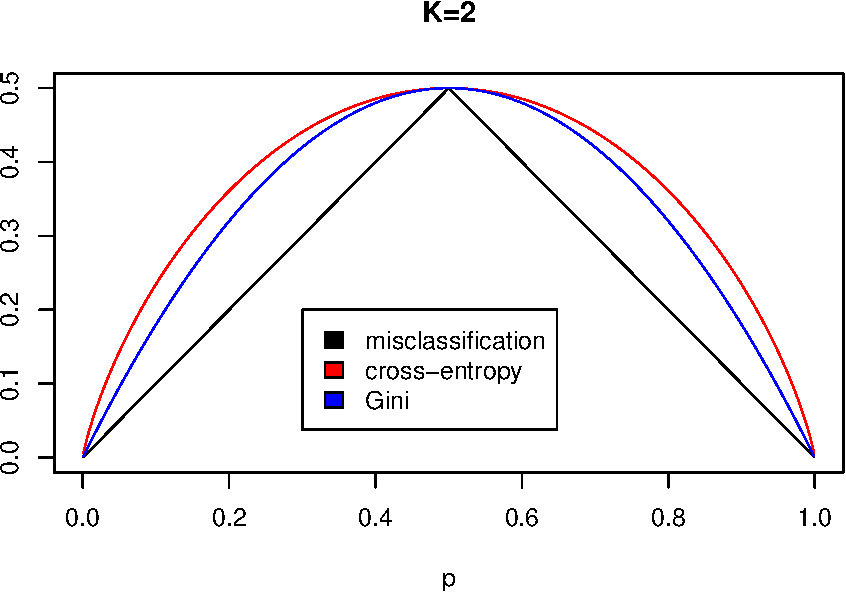
\includegraphics{RecEx2-sol_files/figure-latex/unnamed-chunk-11-1.pdf}

\hypertarget{problem-5}{%
\section{Problem 5}\label{problem-5}}

\begin{enumerate}
\def\labelenumi{\alph{enumi})}
\tightlist
\item
  We sample from the model \(y=x^2+\epsilon\) where
  \(\epsilon \sim \mathcal{N}(0,2^2)\) and
  \(x\in \{-2,-1.9,-1.8,...,3.8,3.9,4\}\). This means that
  \(y \sim \mathcal{N}(x^2,2^2)\). A total of 100 samples from this
  model are generated for each of the 61 \(x\)'s.\\
  See comments in code for further explanations.
\end{enumerate}

\begin{Shaded}
\begin{Highlighting}[]
\FunctionTok{set.seed}\NormalTok{(}\DecValTok{2}\NormalTok{) }\CommentTok{\# to reproduce}

\NormalTok{M }\OtherTok{\textless{}{-}} \DecValTok{100} \CommentTok{\# repeated samplings, x fixed}
\NormalTok{nord }\OtherTok{\textless{}{-}} \DecValTok{20} \CommentTok{\# order of polynomials}

\CommentTok{\#{-}{-}{-}{-}{-}{-}}

\NormalTok{x }\OtherTok{\textless{}{-}} \FunctionTok{seq}\NormalTok{(}\AttributeTok{from =} \SpecialCharTok{{-}}\DecValTok{2}\NormalTok{, }\AttributeTok{to =} \DecValTok{4}\NormalTok{, }\AttributeTok{by =} \FloatTok{0.1}\NormalTok{) }\CommentTok{\#We make a sequence of 61 points, x. These are the points for which we evaluate the function f(x).}

\NormalTok{truefunc }\OtherTok{\textless{}{-}} \ControlFlowTok{function}\NormalTok{(x) \{}
  \FunctionTok{return}\NormalTok{(x}\SpecialCharTok{\^{}}\DecValTok{2}\NormalTok{) }\CommentTok{\#The true f(x)=x\^{}2. }
\NormalTok{\}}
\NormalTok{true\_y }\OtherTok{\textless{}{-}} \FunctionTok{truefunc}\NormalTok{(x) }\CommentTok{\#We find f(x) for each element in vector x.}
\NormalTok{error }\OtherTok{\textless{}{-}} \FunctionTok{matrix}\NormalTok{(}\FunctionTok{rnorm}\NormalTok{(}\FunctionTok{length}\NormalTok{(x) }\SpecialCharTok{*}\NormalTok{ M, }\AttributeTok{mean =} \DecValTok{0}\NormalTok{, }\AttributeTok{sd =} \DecValTok{2}\NormalTok{),}
                \AttributeTok{nrow =}\NormalTok{ M,}
                \AttributeTok{byrow =} \ConstantTok{TRUE}\NormalTok{) }\CommentTok{\#Noise (epsilon) is sampled from a normal distribution and stored in this matrix. Each column corresponds to one value of x.}
\NormalTok{ymat }\OtherTok{\textless{}{-}} \FunctionTok{matrix}\NormalTok{(}\FunctionTok{rep}\NormalTok{(true\_y, M), }\AttributeTok{byrow =}\NormalTok{ T, }\AttributeTok{nrow =}\NormalTok{ M) }\SpecialCharTok{+}\NormalTok{ error  }\CommentTok{\#The 100 samples or the observations are stored in this matrix. Each row is a simulation.}

\CommentTok{\#{-}{-}{-}{-}{-}{-}}

\NormalTok{predictions\_list }\OtherTok{\textless{}{-}} \FunctionTok{lapply}\NormalTok{(}\DecValTok{1}\SpecialCharTok{:}\NormalTok{nord, matrix, }\AttributeTok{data =} \ConstantTok{NA}\NormalTok{, }\AttributeTok{nrow =}\NormalTok{ M, }\AttributeTok{ncol =} \FunctionTok{ncol}\NormalTok{(ymat))}
\ControlFlowTok{for}\NormalTok{(i }\ControlFlowTok{in} \DecValTok{1}\SpecialCharTok{:}\NormalTok{nord)\{}
  \ControlFlowTok{for}\NormalTok{(j }\ControlFlowTok{in} \DecValTok{1}\SpecialCharTok{:}\NormalTok{M)\{}
\NormalTok{    predictions\_list[[i]][j, ] }\OtherTok{\textless{}{-}} \FunctionTok{predict}\NormalTok{(}\FunctionTok{lm}\NormalTok{(ymat[j,] }\SpecialCharTok{\textasciitilde{}} \FunctionTok{poly}\NormalTok{(x, i, }\AttributeTok{raw =} \ConstantTok{TRUE}\NormalTok{))) }\CommentTok{\#Based on the response y\_i and the x\_i\textquotesingle{}s, we fit a polynomial model of degre 1,...,20. This means that we assume y\_i\textasciitilde{}Normal(x\_i\^{}j,0). }
\NormalTok{  \}}
\NormalTok{\}}

\CommentTok{\# Plotting {-}{-}{-}{-}{-}}

\FunctionTok{library}\NormalTok{(tidyverse) }\CommentTok{\# The tidyverse contains ggplot2, as well as tidyr and dplyr, }
\CommentTok{\# which we can use for dataframe manipulation.}

\NormalTok{list\_of\_matrices\_with\_deg\_id }\OtherTok{\textless{}{-}} 
  \FunctionTok{lapply}\NormalTok{(}\DecValTok{1}\SpecialCharTok{:}\NormalTok{nord, }
         \ControlFlowTok{function}\NormalTok{(poly\_degree)\{}\FunctionTok{cbind}\NormalTok{(predictions\_list[[poly\_degree]], }
                                     \AttributeTok{simulation\_num =} \DecValTok{1}\SpecialCharTok{:}\NormalTok{M, poly\_degree)\}}
\NormalTok{         )}
\CommentTok{\# Now predictions\_list is a list with 20 entries, where each entry is a matrix }
\CommentTok{\# with 100 rows, where each row is the predicted polynomial of that degree.}
\CommentTok{\# We also have a column for the simulation number, and a column for polynomial degree.}

\CommentTok{\# Extract each matrix and bind them to one large matrix}
\NormalTok{stacked\_matrices }\OtherTok{\textless{}{-}}  \ConstantTok{NULL}
\ControlFlowTok{for}\NormalTok{ (i }\ControlFlowTok{in} \DecValTok{1}\SpecialCharTok{:}\NormalTok{nord) \{}
\NormalTok{  stacked\_matrices }\OtherTok{\textless{}{-}}
    \FunctionTok{rbind}\NormalTok{(stacked\_matrices, list\_of\_matrices\_with\_deg\_id[[i]])}
\NormalTok{\}}
\NormalTok{stacked\_matrices\_df }\OtherTok{\textless{}{-}} \FunctionTok{as.data.frame}\NormalTok{(stacked\_matrices)}

\CommentTok{\# Convert from wide to long (because that is the best format for ggplot2)}
\NormalTok{long\_predictions\_df }\OtherTok{\textless{}{-}} \FunctionTok{pivot\_longer}\NormalTok{(stacked\_matrices\_df, }
                                    \SpecialCharTok{!}\FunctionTok{c}\NormalTok{(simulation\_num, poly\_degree), }
                                    \AttributeTok{values\_to =} \StringTok{"y"}\NormalTok{)}

\CommentTok{\# Now we can use ggplot2!}
\CommentTok{\# We just want to plot for degrees 1, 2, 10 and 20.}

\NormalTok{plotting\_df }\OtherTok{\textless{}{-}} \FunctionTok{cbind}\NormalTok{(long\_predictions\_df, }\AttributeTok{x =}\NormalTok{ x) }\SpecialCharTok{\%\textgreater{}\%} \CommentTok{\# adding the x{-}vector to the dataframe}
  \FunctionTok{filter}\NormalTok{(poly\_degree }\SpecialCharTok{\%in\%} \FunctionTok{c}\NormalTok{(}\DecValTok{1}\NormalTok{, }\DecValTok{2}\NormalTok{, }\DecValTok{10}\NormalTok{, }\DecValTok{20}\NormalTok{)) }\CommentTok{\# Select only the predictions using degree 1, 2, 10 or 20}

\FunctionTok{ggplot}\NormalTok{(plotting\_df, }\FunctionTok{aes}\NormalTok{(}\AttributeTok{x =}\NormalTok{ x, }\AttributeTok{y =}\NormalTok{ y, }\AttributeTok{group =}\NormalTok{ simulation\_num)) }\SpecialCharTok{+}
  \FunctionTok{geom\_line}\NormalTok{(}\FunctionTok{aes}\NormalTok{(}\AttributeTok{color =}\NormalTok{ simulation\_num)) }\SpecialCharTok{+}
  \FunctionTok{geom\_line}\NormalTok{(}\FunctionTok{aes}\NormalTok{(}\AttributeTok{x =}\NormalTok{ x, }\AttributeTok{y =}\NormalTok{ x}\SpecialCharTok{\^{}}\DecValTok{2}\NormalTok{), }\AttributeTok{size =} \FloatTok{1.5}\NormalTok{) }\SpecialCharTok{+}
  \FunctionTok{facet\_wrap}\NormalTok{(}\SpecialCharTok{\textasciitilde{}}\NormalTok{ poly\_degree) }\SpecialCharTok{+}
  \FunctionTok{theme\_bw}\NormalTok{() }\SpecialCharTok{+}
  \FunctionTok{theme}\NormalTok{(}\AttributeTok{legend.position =} \StringTok{"none"}\NormalTok{)}
\end{Highlighting}
\end{Shaded}

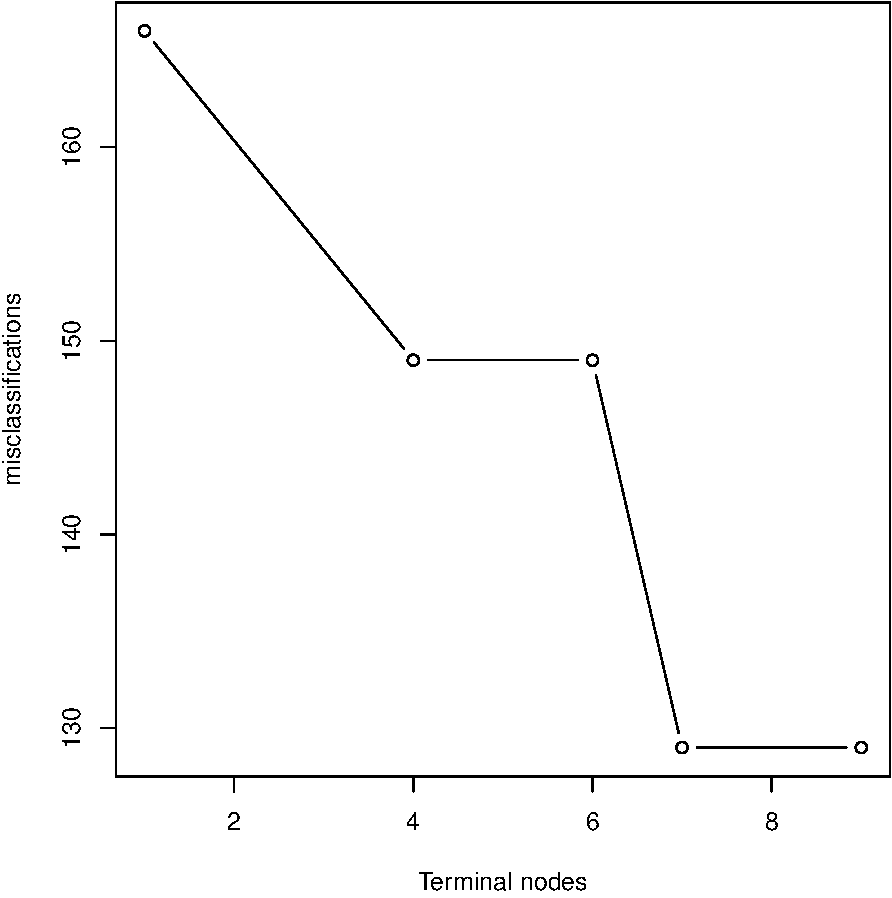
\includegraphics{RecEx2-sol_files/figure-latex/unnamed-chunk-12-1.pdf}

The upper left plot shows 100 predictions when we assume that \(y\) is a
linear function of \(x\), the upper right plot hows 100 predictions when
we assume that \(y\) is function of poynomials up to \(x^2\), the lower
left plot shows 100 predictions when we assume \(y\) is a function of
polynomials up to \(x^{10}\) and the lower right plot shows 100
predictions when assuming \(y\) is a function of polynomials up to
\(x^{20}\).

\begin{enumerate}
\def\labelenumi{\alph{enumi})}
\setcounter{enumi}{1}
\tightlist
\item
  Run the code attached and consider the following plots:
\end{enumerate}

\begin{Shaded}
\begin{Highlighting}[]
\FunctionTok{set.seed}\NormalTok{(}\DecValTok{2}\NormalTok{) }\CommentTok{\# to reproduce}
\NormalTok{M }\OtherTok{\textless{}{-}} \DecValTok{100} \CommentTok{\# repeated samplings,x fixed but new errors}
\NormalTok{nord }\OtherTok{\textless{}{-}} \DecValTok{20}

\NormalTok{x }\OtherTok{\textless{}{-}} \FunctionTok{seq}\NormalTok{(}\AttributeTok{from =} \SpecialCharTok{{-}}\DecValTok{2}\NormalTok{, }\AttributeTok{to =} \DecValTok{4}\NormalTok{, }\AttributeTok{by =} \FloatTok{0.1}\NormalTok{)}
\NormalTok{truefunc }\OtherTok{\textless{}{-}} \ControlFlowTok{function}\NormalTok{(x)\{}
  \FunctionTok{return}\NormalTok{(x}\SpecialCharTok{\^{}}\DecValTok{2}\NormalTok{)}
\NormalTok{\}}
\NormalTok{true\_y }\OtherTok{\textless{}{-}} \FunctionTok{truefunc}\NormalTok{(x)}
\NormalTok{error }\OtherTok{\textless{}{-}} \FunctionTok{matrix}\NormalTok{(}\FunctionTok{rnorm}\NormalTok{(}\FunctionTok{length}\NormalTok{(x)}\SpecialCharTok{*}\NormalTok{M, }\AttributeTok{mean =} \DecValTok{0}\NormalTok{, }\AttributeTok{sd =} \DecValTok{2}\NormalTok{), }\AttributeTok{nrow =}\NormalTok{ M, }\AttributeTok{byrow =} \ConstantTok{TRUE}\NormalTok{)}
\NormalTok{testerror }\OtherTok{\textless{}{-}} \FunctionTok{matrix}\NormalTok{(}\FunctionTok{rnorm}\NormalTok{(}\FunctionTok{length}\NormalTok{(x)}\SpecialCharTok{*}\NormalTok{M, }\AttributeTok{mean =} \DecValTok{0}\NormalTok{, }\AttributeTok{sd =} \DecValTok{2}\NormalTok{), }\AttributeTok{nrow =}\NormalTok{ M, }\AttributeTok{byrow =} \ConstantTok{TRUE}\NormalTok{)}
\NormalTok{ymat }\OtherTok{\textless{}{-}} \FunctionTok{matrix}\NormalTok{(}\FunctionTok{rep}\NormalTok{(true\_y, M), }\AttributeTok{byrow =}\NormalTok{ T, }\AttributeTok{nrow =}\NormalTok{ M) }\SpecialCharTok{+}\NormalTok{ error}
\NormalTok{testymat }\OtherTok{\textless{}{-}} \FunctionTok{matrix}\NormalTok{(}\FunctionTok{rep}\NormalTok{(true\_y, M), }\AttributeTok{byrow=}\NormalTok{T, }\AttributeTok{nrow=}\NormalTok{M) }\SpecialCharTok{+}\NormalTok{ testerror}

\NormalTok{predictions\_list }\OtherTok{\textless{}{-}} \FunctionTok{lapply}\NormalTok{(}\DecValTok{1}\SpecialCharTok{:}\NormalTok{nord, matrix, }\AttributeTok{data =} \ConstantTok{NA}\NormalTok{, }\AttributeTok{nrow =}\NormalTok{ M, }\AttributeTok{ncol =} \FunctionTok{ncol}\NormalTok{(ymat))}
\ControlFlowTok{for}\NormalTok{(i }\ControlFlowTok{in} \DecValTok{1}\SpecialCharTok{:}\NormalTok{nord)\{}
  \ControlFlowTok{for}\NormalTok{(j }\ControlFlowTok{in} \DecValTok{1}\SpecialCharTok{:}\NormalTok{M)\{}
\NormalTok{    predictions\_list[[i]][j, ] }\OtherTok{\textless{}{-}} \FunctionTok{predict}\NormalTok{(}\FunctionTok{lm}\NormalTok{(ymat[j,] }\SpecialCharTok{\textasciitilde{}} \FunctionTok{poly}\NormalTok{(x, i, }\AttributeTok{raw =} \ConstantTok{TRUE}\NormalTok{)))}
\NormalTok{  \}}
\NormalTok{\}}

\NormalTok{trainMSE }\OtherTok{\textless{}{-}} \FunctionTok{lapply}\NormalTok{(}\DecValTok{1}\SpecialCharTok{:}\NormalTok{nord, }
                   \ControlFlowTok{function}\NormalTok{(poly\_degree)\{}
                     \FunctionTok{rowMeans}\NormalTok{((predictions\_list[[poly\_degree]] }\SpecialCharTok{{-}}\NormalTok{ ymat)}\SpecialCharTok{\^{}}\DecValTok{2}\NormalTok{)\}}
\NormalTok{                   )}
\NormalTok{testMSE }\OtherTok{\textless{}{-}} \FunctionTok{lapply}\NormalTok{(}\DecValTok{1}\SpecialCharTok{:}\NormalTok{nord, }
                  \ControlFlowTok{function}\NormalTok{(poly\_degree)\{}
                    \FunctionTok{rowMeans}\NormalTok{((predictions\_list[[poly\_degree]] }\SpecialCharTok{{-}}\NormalTok{ testymat)}\SpecialCharTok{\^{}}\DecValTok{2}\NormalTok{)\}}
\NormalTok{                  )}

\CommentTok{\# Plotting {-}{-}{-}{-}{-}}
\FunctionTok{library}\NormalTok{(tidyverse) }\CommentTok{\# The tidyverse contains ggplot2, as well as tidyr and dplyr, }
\CommentTok{\# which we can use for dataframe manipulation.}

\CommentTok{\# Convert each matrix in the list form wide to long (because that is the best format for ggplot2)}
\NormalTok{list\_train\_MSE }\OtherTok{\textless{}{-}} \FunctionTok{lapply}\NormalTok{(}\DecValTok{1}\SpecialCharTok{:}\NormalTok{nord, }\ControlFlowTok{function}\NormalTok{(poly\_degree) }\FunctionTok{cbind}\NormalTok{(}\AttributeTok{error =}\NormalTok{ trainMSE[[poly\_degree]], }
\NormalTok{                                                             poly\_degree, }
                                                             \AttributeTok{error\_type =} \StringTok{"train"}\NormalTok{,}
                                                             \AttributeTok{simulation\_num =} \DecValTok{1}\SpecialCharTok{:}\NormalTok{M))}
\NormalTok{list\_test\_MSE }\OtherTok{\textless{}{-}} \FunctionTok{lapply}\NormalTok{(}\DecValTok{1}\SpecialCharTok{:}\NormalTok{nord, }\ControlFlowTok{function}\NormalTok{(poly\_degree) }\FunctionTok{cbind}\NormalTok{(}\AttributeTok{error =}\NormalTok{ testMSE[[poly\_degree]], }
\NormalTok{                                                            poly\_degree, }
                                                            \AttributeTok{error\_type =} \StringTok{"test"}\NormalTok{, }
                                                            \AttributeTok{simulation\_num =} \DecValTok{1}\SpecialCharTok{:}\NormalTok{M))}

\CommentTok{\# Now predictions\_list is a list with 20 entries, where each entry is a matrix }
\CommentTok{\# with 100 rows, where each row is the predicted polynomial of that degree.}

\NormalTok{stacked\_train }\OtherTok{\textless{}{-}} \ConstantTok{NULL}
\ControlFlowTok{for}\NormalTok{ (i }\ControlFlowTok{in} \DecValTok{1}\SpecialCharTok{:}\NormalTok{nord) \{}
\NormalTok{  stacked\_train }\OtherTok{\textless{}{-}}
    \FunctionTok{rbind}\NormalTok{(stacked\_train, list\_train\_MSE[[i]])}
\NormalTok{\}}
\NormalTok{stacked\_test }\OtherTok{\textless{}{-}} \ConstantTok{NULL}
\ControlFlowTok{for}\NormalTok{ (i }\ControlFlowTok{in} \DecValTok{1}\SpecialCharTok{:}\NormalTok{nord) \{}
\NormalTok{  stacked\_test }\OtherTok{\textless{}{-}}
    \FunctionTok{rbind}\NormalTok{(stacked\_test, list\_test\_MSE[[i]])}
\NormalTok{\}}

\NormalTok{stacked\_errors\_df }\OtherTok{\textless{}{-}} \FunctionTok{as.data.frame}\NormalTok{(}\FunctionTok{rbind}\NormalTok{(stacked\_train, stacked\_test))}
\CommentTok{\# This is already on long format. }
\NormalTok{stacked\_errors\_df}\SpecialCharTok{$}\NormalTok{error }\OtherTok{\textless{}{-}} \FunctionTok{as.numeric}\NormalTok{(stacked\_errors\_df}\SpecialCharTok{$}\NormalTok{error)}
\NormalTok{stacked\_errors\_df}\SpecialCharTok{$}\NormalTok{simulation\_num }\OtherTok{\textless{}{-}} \FunctionTok{as.integer}\NormalTok{(stacked\_errors\_df}\SpecialCharTok{$}\NormalTok{simulation\_num)}
\NormalTok{stacked\_errors\_df}\SpecialCharTok{$}\NormalTok{poly\_degree }\OtherTok{\textless{}{-}} \FunctionTok{as.integer}\NormalTok{(stacked\_errors\_df}\SpecialCharTok{$}\NormalTok{poly\_degree)}

\NormalTok{p.all\_lines }\OtherTok{\textless{}{-}} \FunctionTok{ggplot}\NormalTok{(}\AttributeTok{data =}\NormalTok{ stacked\_errors\_df, }\FunctionTok{aes}\NormalTok{(}\AttributeTok{x =}\NormalTok{ poly\_degree, }\AttributeTok{y =}\NormalTok{ error, }\AttributeTok{group =}\NormalTok{ simulation\_num)) }\SpecialCharTok{+}
  \FunctionTok{geom\_line}\NormalTok{(}\FunctionTok{aes}\NormalTok{(}\AttributeTok{color =}\NormalTok{ simulation\_num)) }\SpecialCharTok{+}
  \FunctionTok{facet\_wrap}\NormalTok{(}\SpecialCharTok{\textasciitilde{}}\NormalTok{ error\_type) }\SpecialCharTok{+}
  \FunctionTok{xlab}\NormalTok{(}\StringTok{"Polynomial degree"}\NormalTok{) }\SpecialCharTok{+}
  \FunctionTok{ylab}\NormalTok{(}\StringTok{"MSE"}\NormalTok{) }\SpecialCharTok{+}
  \FunctionTok{theme\_bw}\NormalTok{() }\SpecialCharTok{+}
  \FunctionTok{theme}\NormalTok{(}\AttributeTok{legend.position =} \StringTok{"none"}\NormalTok{)}

\NormalTok{p.bars }\OtherTok{\textless{}{-}} \FunctionTok{ggplot}\NormalTok{(stacked\_errors\_df, }\FunctionTok{aes}\NormalTok{(}\AttributeTok{x =} \FunctionTok{as.factor}\NormalTok{(poly\_degree), }\AttributeTok{y =}\NormalTok{ error)) }\SpecialCharTok{+}
  \FunctionTok{geom\_boxplot}\NormalTok{(}\FunctionTok{aes}\NormalTok{(}\AttributeTok{fill =}\NormalTok{ error\_type)) }\SpecialCharTok{+}
  \FunctionTok{scale\_fill\_discrete}\NormalTok{(}\AttributeTok{name =} \StringTok{"Error type"}\NormalTok{) }\SpecialCharTok{+}
  \FunctionTok{xlab}\NormalTok{(}\StringTok{"Polynomial degree"}\NormalTok{) }\SpecialCharTok{+}
  \FunctionTok{ylab}\NormalTok{(}\StringTok{"MSE"}\NormalTok{) }\SpecialCharTok{+}
  \FunctionTok{theme\_bw}\NormalTok{()}

\CommentTok{\# Here we find the average test error and training error across the repeated simulations. }
\CommentTok{\# The symbol "\%\textgreater{}\%" is called a pipe, and comes from the tidyverse packages, }
\CommentTok{\# which provide convenient functions for working with data frames.}
\NormalTok{means\_across\_simulations }\OtherTok{\textless{}{-}}\NormalTok{ stacked\_errors\_df }\SpecialCharTok{\%\textgreater{}\%} 
  \FunctionTok{group\_by}\NormalTok{(error\_type, poly\_degree) }\SpecialCharTok{\%\textgreater{}\%} 
  \FunctionTok{summarise}\NormalTok{(}\AttributeTok{mean =} \FunctionTok{mean}\NormalTok{(error))}
\end{Highlighting}
\end{Shaded}

\begin{verbatim}
## `summarise()` has grouped output by 'error_type'. You can override using the `.groups` argument.
\end{verbatim}

\begin{Shaded}
\begin{Highlighting}[]
\NormalTok{p.means }\OtherTok{\textless{}{-}} \FunctionTok{ggplot}\NormalTok{(means\_across\_simulations, }\FunctionTok{aes}\NormalTok{(}\AttributeTok{x =}\NormalTok{ poly\_degree, }\AttributeTok{y =}\NormalTok{ mean)) }\SpecialCharTok{+}
  \FunctionTok{geom\_line}\NormalTok{(}\FunctionTok{aes}\NormalTok{(}\AttributeTok{color =}\NormalTok{ error\_type)) }\SpecialCharTok{+}
  \FunctionTok{scale\_color\_discrete}\NormalTok{(}\AttributeTok{name =} \StringTok{"Error type"}\NormalTok{) }\SpecialCharTok{+}
  \FunctionTok{xlab}\NormalTok{(}\StringTok{"Polynomial degree"}\NormalTok{) }\SpecialCharTok{+}
  \FunctionTok{ylab}\NormalTok{(}\StringTok{"MSE"}\NormalTok{) }\SpecialCharTok{+}
  \FunctionTok{theme\_bw}\NormalTok{()}

\FunctionTok{library}\NormalTok{(patchwork) }\CommentTok{\# The library patchwork is the best way of combining ggplot2 objects. }
\CommentTok{\# You could also use the function ggarrange from the ggpubr package.}

\NormalTok{p.all\_lines }\SpecialCharTok{/}\NormalTok{ (p.bars }\SpecialCharTok{+}\NormalTok{ p.means)}
\end{Highlighting}
\end{Shaded}

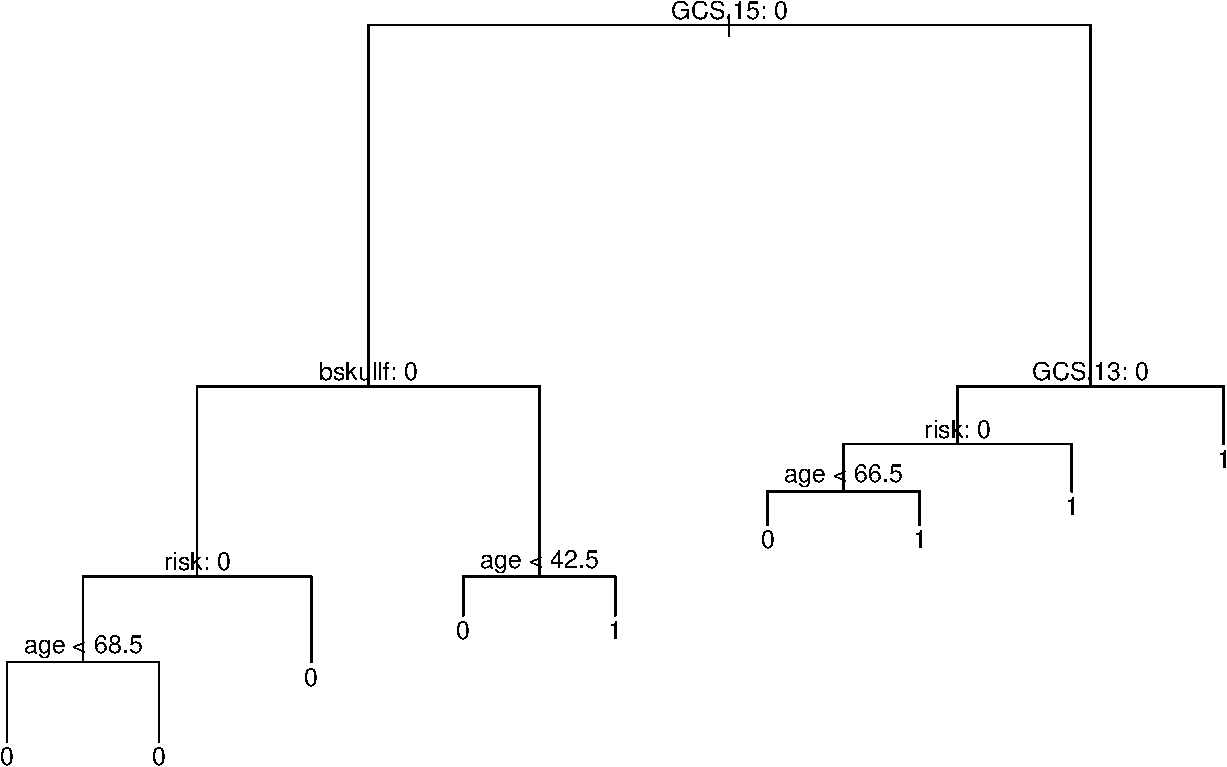
\includegraphics{RecEx2-sol_files/figure-latex/unnamed-chunk-13-1.pdf}

The plots show that the test MSE in general is larger than the train
MSE. This is reasonable. The fitted model is fitted based on the
training set. Thus, the error will be smaller for the train data than
for the test data. Furthermore, the plots show that the difference
between the MSE for the test set and the training set increases when the
degree of the polynomial increases. When the degree of the polynomial
increases, we get a more flexible model. The fitted curve will try to
pass through the training data if possible, which typically leads to an
overfitted model that performs bad for test data.

\begin{itemize}
\tightlist
\item
  We observe that poly 2 gives the smallest mean testMSE, while poly 20
  gives the smallest trainMSE. Based on these plots, we would choose
  poly 2 for prediction of a new value of \(y\), as the testMSE tells us
  more about how the model performs on data not used to train the model.
\end{itemize}

\begin{enumerate}
\def\labelenumi{\alph{enumi})}
\setcounter{enumi}{2}
\tightlist
\item
  Run the code and consider the following plots:
\end{enumerate}

\begin{Shaded}
\begin{Highlighting}[]
\NormalTok{meanmat }\OtherTok{\textless{}{-}} \FunctionTok{matrix}\NormalTok{(}\AttributeTok{ncol =} \FunctionTok{length}\NormalTok{(x), }\AttributeTok{nrow =}\NormalTok{ nord)}
\NormalTok{varmat }\OtherTok{\textless{}{-}} \FunctionTok{matrix}\NormalTok{(}\AttributeTok{ncol =} \FunctionTok{length}\NormalTok{(x), }\AttributeTok{nrow =}\NormalTok{ nord)}
\ControlFlowTok{for}\NormalTok{ (j }\ControlFlowTok{in} \DecValTok{1}\SpecialCharTok{:}\NormalTok{nord)\{}
\NormalTok{  meanmat[j,] }\OtherTok{\textless{}{-}} \FunctionTok{apply}\NormalTok{(predictions\_list[[j]], }\DecValTok{2}\NormalTok{, mean) }\CommentTok{\# we now take the mean over the M simulations {-} to mimic E and Var at each x value and each poly model}
\NormalTok{  varmat[j,] }\OtherTok{\textless{}{-}} \FunctionTok{apply}\NormalTok{(predictions\_list[[j]], }\DecValTok{2}\NormalTok{, var)}
\NormalTok{\}}

\CommentTok{\# nord times length(x)}
\NormalTok{bias2mat }\OtherTok{\textless{}{-}}\NormalTok{ (meanmat }\SpecialCharTok{{-}} \FunctionTok{matrix}\NormalTok{(}\FunctionTok{rep}\NormalTok{(true\_y, nord), }\AttributeTok{byrow =} \ConstantTok{TRUE}\NormalTok{, }\AttributeTok{nrow =}\NormalTok{ nord))}\SpecialCharTok{\^{}}\DecValTok{2} \CommentTok{\#here the truth is finally used!}

\NormalTok{df }\OtherTok{\textless{}{-}} \FunctionTok{data.frame}\NormalTok{(}\AttributeTok{x =} \FunctionTok{rep}\NormalTok{(x, }\AttributeTok{each =}\NormalTok{ nord), }\AttributeTok{poly\_degree =} \FunctionTok{rep}\NormalTok{(}\DecValTok{1}\SpecialCharTok{:}\NormalTok{nord, }\FunctionTok{length}\NormalTok{(x)), }
                 \AttributeTok{bias2 =} \FunctionTok{c}\NormalTok{(bias2mat), }\AttributeTok{variance =} \FunctionTok{c}\NormalTok{(varmat), }
                 \AttributeTok{irreducible\_error =} \FunctionTok{rep}\NormalTok{(}\DecValTok{4}\NormalTok{, }\FunctionTok{prod}\NormalTok{(}\FunctionTok{dim}\NormalTok{(varmat)))) }\CommentTok{\#irr is just 1}

\NormalTok{df}\SpecialCharTok{$}\NormalTok{total }\OtherTok{\textless{}{-}}\NormalTok{ df}\SpecialCharTok{$}\NormalTok{bias2 }\SpecialCharTok{+}\NormalTok{ df}\SpecialCharTok{$}\NormalTok{variance }\SpecialCharTok{+}\NormalTok{ df}\SpecialCharTok{$}\NormalTok{irreducible\_error}

\NormalTok{df\_long }\OtherTok{\textless{}{-}} \FunctionTok{pivot\_longer}\NormalTok{(df, }\AttributeTok{cols =} \SpecialCharTok{!}\FunctionTok{c}\NormalTok{(x, poly\_degree), }\AttributeTok{names\_to =} \StringTok{"type"}\NormalTok{) }

\NormalTok{df\_select\_poly }\OtherTok{\textless{}{-}} \FunctionTok{filter}\NormalTok{(df\_long, poly\_degree }\SpecialCharTok{\%in\%} \FunctionTok{c}\NormalTok{(}\DecValTok{1}\NormalTok{, }\DecValTok{2}\NormalTok{, }\DecValTok{10}\NormalTok{, }\DecValTok{20}\NormalTok{))}

\FunctionTok{ggplot}\NormalTok{(df\_select\_poly, }\FunctionTok{aes}\NormalTok{(}\AttributeTok{x =}\NormalTok{ x, }\AttributeTok{y =}\NormalTok{ value, }\AttributeTok{group =}\NormalTok{ type)) }\SpecialCharTok{+}
  \FunctionTok{geom\_line}\NormalTok{(}\FunctionTok{aes}\NormalTok{(}\AttributeTok{color =}\NormalTok{ type)) }\SpecialCharTok{+}
  \FunctionTok{facet\_wrap}\NormalTok{(}\SpecialCharTok{\textasciitilde{}}\NormalTok{poly\_degree, }\AttributeTok{scales =} \StringTok{"free"}\NormalTok{, }\AttributeTok{labeller =}\NormalTok{ label\_both) }\SpecialCharTok{+}
  \FunctionTok{theme\_bw}\NormalTok{()}
\end{Highlighting}
\end{Shaded}

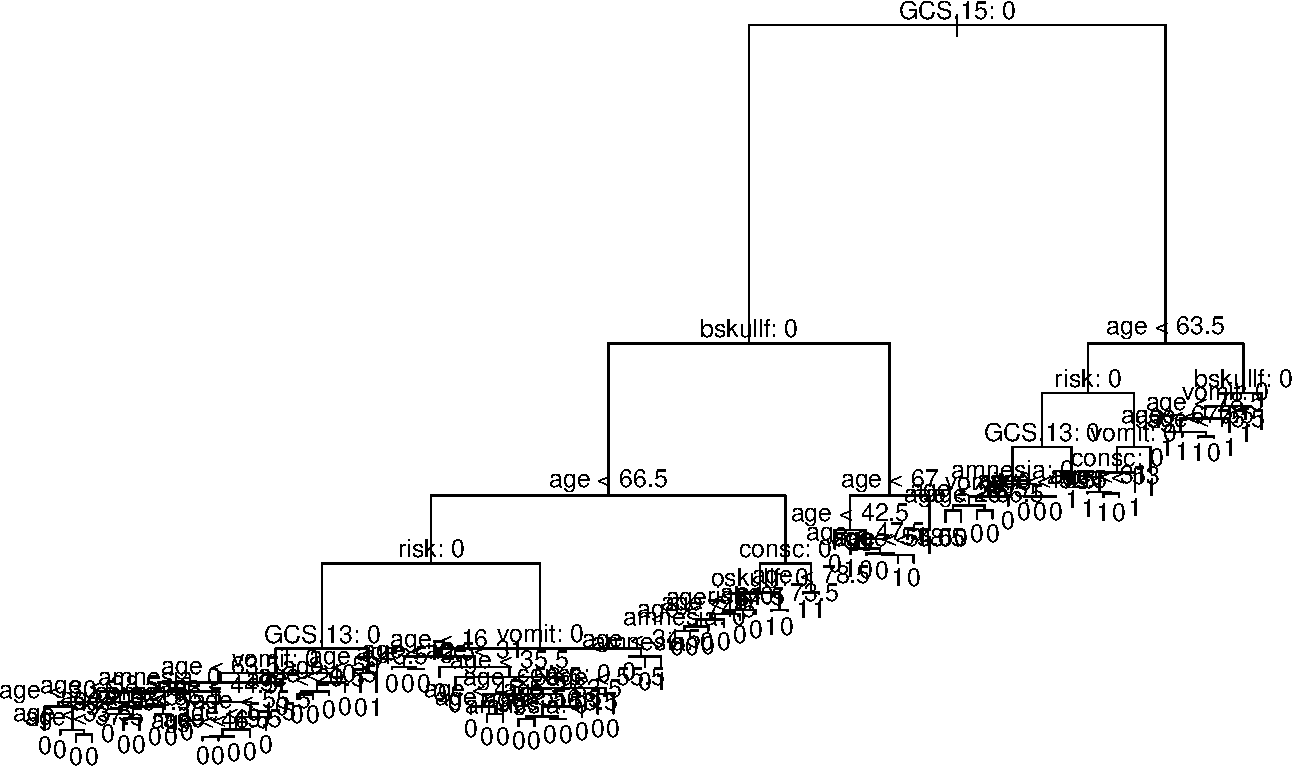
\includegraphics{RecEx2-sol_files/figure-latex/unnamed-chunk-14-1.pdf}

We see that the irriducible error remains constant with the complexity
of the model and the variance (purple) increases with the complexity. A
linear model gives variance close to zero, while a polynomial of degree
20 gives variance close to 1 (larger at the borders). A more complex
model is more flexible as it can turn up and down and change direction
fast. This leads to larger variance. (Look at the plot in 2a, there is a
larger variety of curves you can make when the degree is 20 compared to
if the degree is 1.).

Further, we see that the bias is large for poly1, the linear model. The
linear model is quite rigid, so if the true underlying model is
non-linear, we typically get large deviations between the fitted line
and the training data. If we study the first plot, it seems like the
fitted line goes through the training data in \(x=-1\) and \(x=3\) as
the bias is close to zero here (this is confirmed by looking at the
upper left plot in 2a).

The polynomial models with degree larger than one lead to lower bias.
Recall that this is the training bias: The polynomial models will try to
pass through the training points if possible, and when the degree of the
polynomial is large they are able to do so because they have large
flexibility compared to a linear model.

\begin{Shaded}
\begin{Highlighting}[]
\NormalTok{df\_select\_x }\OtherTok{\textless{}{-}} \FunctionTok{filter}\NormalTok{(df\_long, x }\SpecialCharTok{\%in\%} \FunctionTok{c}\NormalTok{(}\SpecialCharTok{{-}}\DecValTok{1}\NormalTok{, }\FloatTok{0.5}\NormalTok{, }\DecValTok{2}\NormalTok{, }\FloatTok{3.5}\NormalTok{))}

\FunctionTok{ggplot}\NormalTok{(df\_select\_x, }\FunctionTok{aes}\NormalTok{(}\AttributeTok{x =}\NormalTok{ poly\_degree, }\AttributeTok{y =}\NormalTok{ value, }\AttributeTok{group =}\NormalTok{ type)) }\SpecialCharTok{+}
  \FunctionTok{geom\_line}\NormalTok{(}\FunctionTok{aes}\NormalTok{(}\AttributeTok{color =}\NormalTok{ type)) }\SpecialCharTok{+}
  \FunctionTok{facet\_wrap}\NormalTok{(}\SpecialCharTok{\textasciitilde{}}\NormalTok{x, }\AttributeTok{scales =} \StringTok{"free"}\NormalTok{, }\AttributeTok{labeller =}\NormalTok{ label\_both) }\SpecialCharTok{+}
  \FunctionTok{theme\_bw}\NormalTok{()}
\end{Highlighting}
\end{Shaded}

\includegraphics{RecEx2-sol_files/figure-latex/2bbiasvariance2-1.pdf}

Compare to Figures in 2.12 on page 36 in ISL (our textbook).

\begin{enumerate}
\def\labelenumi{\alph{enumi})}
\setcounter{enumi}{3}
\tightlist
\item
  To change \(f(x)\), replace
\end{enumerate}

\begin{Shaded}
\begin{Highlighting}[]
\NormalTok{truefunc}\OtherTok{=}\ControlFlowTok{function}\NormalTok{(x) }\FunctionTok{return}\NormalTok{(x}\SpecialCharTok{\^{}}\DecValTok{2}\NormalTok{)}
\end{Highlighting}
\end{Shaded}

by for example

\begin{Shaded}
\begin{Highlighting}[]
\NormalTok{truefunc}\OtherTok{=}\ControlFlowTok{function}\NormalTok{(x) }\FunctionTok{return}\NormalTok{(x}\SpecialCharTok{\^{}}\DecValTok{4}\NormalTok{)}
\end{Highlighting}
\end{Shaded}

or

\begin{Shaded}
\begin{Highlighting}[]
\NormalTok{truefunc}\OtherTok{=}\ControlFlowTok{function}\NormalTok{(x) }\FunctionTok{return}\NormalTok{(}\FunctionTok{exp}\NormalTok{(}\DecValTok{2}\SpecialCharTok{*}\NormalTok{x))}
\end{Highlighting}
\end{Shaded}

and rerun the code. Study the results.

If you want to set the variance to 1 for example, set \(sd=1\) in these
parts of the code in 2a and 2b:

\begin{Shaded}
\begin{Highlighting}[]
\NormalTok{rnorm(length(x)*M, mean=0, sd=1)}
\end{Highlighting}
\end{Shaded}

Also change the following part in 2c:

\begin{Shaded}
\begin{Highlighting}[]
\NormalTok{df }\OtherTok{\textless{}{-}} \FunctionTok{data.frame}\NormalTok{(}\AttributeTok{x =} \FunctionTok{rep}\NormalTok{(x, }\AttributeTok{each =}\NormalTok{ nord), }\AttributeTok{poly\_degree =} \FunctionTok{rep}\NormalTok{(}\DecValTok{1}\SpecialCharTok{:}\NormalTok{nord, }\FunctionTok{length}\NormalTok{(x)), }
                 \AttributeTok{bias2 =} \FunctionTok{c}\NormalTok{(bias2mat), }\AttributeTok{variance =} \FunctionTok{c}\NormalTok{(varmat), }
                 \AttributeTok{irreducible\_error =} \FunctionTok{rep}\NormalTok{(}\DecValTok{4}\NormalTok{, }\FunctionTok{prod}\NormalTok{(}\FunctionTok{dim}\NormalTok{(varmat)))) }\CommentTok{\#irr is just 1}
\end{Highlighting}
\end{Shaded}

to get correct plots of the irreducible error. Here,
\texttt{rep(4,prod(dim(varmat)))} is replaced by
\texttt{rep(1,prod(dim(varmat)))}.

\hypertarget{r-packages}{%
\section{\texorpdfstring{ R packages}{ R packages}}\label{r-packages}}

If you want to look at the .Rmd file and \texttt{knit} it, you need to
first install the following packages (only once).

\begin{Shaded}
\begin{Highlighting}[]
\FunctionTok{install.packages}\NormalTok{(}\StringTok{"ggplot2"}\NormalTok{)}
\FunctionTok{install.packages}\NormalTok{(}\StringTok{"gamlss.data"}\NormalTok{)}
\FunctionTok{install.packages}\NormalTok{(}\StringTok{"tidyverse"}\NormalTok{)}
\FunctionTok{install.packages}\NormalTok{(}\StringTok{"GGally"}\NormalTok{)}
\FunctionTok{install.packages}\NormalTok{(}\StringTok{"Matrix"}\NormalTok{)}
\FunctionTok{install.packages}\NormalTok{(}\StringTok{"patchwork"}\NormalTok{)}
\end{Highlighting}
\end{Shaded}

\begin{Shaded}
\begin{Highlighting}[]
\FunctionTok{installed.packages}\NormalTok{()[}\FunctionTok{names}\NormalTok{(}\FunctionTok{sessionInfo}\NormalTok{()}\SpecialCharTok{$}\NormalTok{otherPkgs), }\StringTok{"Version"}\NormalTok{]}
\end{Highlighting}
\end{Shaded}

\begin{verbatim}
##   forcats   stringr     dplyr     purrr     readr     tidyr    tibble tidyverse patchwork      MASS 
##   "0.5.2"   "1.4.1"  "1.0.10"   "0.3.5"   "2.1.3"   "1.2.1"   "3.1.8"   "1.3.2"   "1.1.2"  "7.3-57" 
##    GGally   ggplot2      ISLR     knitr 
##   "2.1.2"   "3.3.6"     "1.4"    "1.40"
\end{verbatim}

\end{document}
